\subsection{Results of Topology Optimization}
Results of the topology optimization process can be seen in figure \ref{fig: topyStar}. Here, a voxelized star was given as input. We set the voxels in the star's points as fixtures, while we set a load in the middle, in the direction normal to the plane of the star. As can be seen, the optimization process "cuts" away unnecessary material in-between the corners and even in the middle of the material, returning an optimally stiff structure for the chosen remaining volume fraction. 

The optimized voxel grid is written into a {\it.vtk} file. Note that the eye-catching voxel shape is a result of the discretization step to solve the topology optimization. From a physical point of view a smooth surface of this shape needs no comment. The next part of the pipeline reconstructs a smooth surface, and converts it back to the CAD world. 
\begin{figure}
\centering
\begin{subfigure}[c]{.2\linewidth}
\centering
  
\includegraphics[width=.9\linewidth]{Pictures/TopOp/Star_Optimized0_Trans.png}
\end{subfigure}%
~
\begin{subfigure}[c]{.2\linewidth}
\centering
  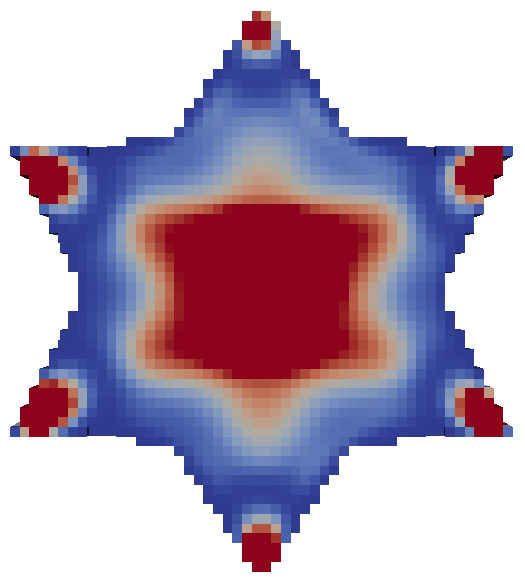
\includegraphics[width=.9\linewidth]{Pictures/TopOp/Star_Optimized2_Trans.png}
\end{subfigure}
~
\begin{subfigure}[c]{.2\linewidth}
\centering
  
\includegraphics[width=.9\linewidth]{Pictures/TopOp/Star_Optimized4_Trans.png}
\end{subfigure}
~
\begin{subfigure}[c]{.2\linewidth}
\centering
  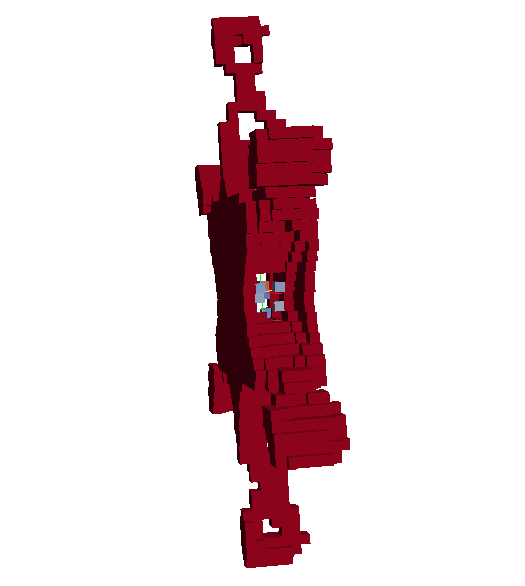
\includegraphics[width=.9\linewidth]{Pictures/TopOp/Star_Optimized5_Trans.png}
\end{subfigure}
\caption{Topology Optimization by ToPy \cite{ToPy}, with minimum compliance. \emph{From left to right}: increasing number of SIMP iterations until convergence. The star-shaped structure was given by an STL-file which was processed into input readable by ToPy, with fixtures in the corners, and a load in the middle. Throughout the SIMP iterations, one can see how material from the less dense regions (blue) is concentrated into denser regions (red) that carry the load. The last picture gives a rotated view, to illustrate how material has been eliminated even from the inside of the star. } %which volume fraction?
\label{fig: topyStar}
\end{figure}
